\section{Конструкторский раздел \hfill}
\vspace{\baselineskip}

В данном разделе описывается метод поиска по словарю при ограничении на значение признака, заданном при помощи лингвистической переменной, а также приводятся разработанные алгоритмы бинарного поиска и получения объектов по заданному в вопросе на естественном языке ограничению.

\vspace{\baselineskip}
\subsection{Метод поиска по словарю при ограничении на значение признака, заданном при помощи лингвистической переменной}
\vspace{\baselineskip}

Этапы метода поиска по словарю при ограничении на значение признака, заданном при помощи лингвистической переменной:
\begin{enumerate}[label=\arabic*)]
\item выполнить графематический анализ входного вопроса --- предложения на русском языке;
\item выполнить морфологический анализ слов из вопроса;
\item проверить наличие в вопросе указания на объект --- планету --- и на Землю;
\item выделить терм и квантификаторы;
\item сформировать ограничение на диапазон значений расстояния соответсвенно выделенным терму и квантификаторам;
\item выполнить поиск в словаре соответственно сформированным ограничениям;
\item подготовить результат к выводу в виде текста на естественном языке.
\end{enumerate}

\vspace{\baselineskip}
\subsection{Разработка алгоритмов} 
\vspace{\baselineskip}

На рисунке \ref{fig:bin-search} приведена схема алгоритма бинарного поиска в словаре. 
На рисунке \ref{fig:not-very} приведены схемы алгоритмов получения объекта по значению функции принадлежности, а также расчета функций принадлежности для квантификаторов <<не>> и <<очень>>.
На рисунках \ref{fig:get1}--\ref{fig:get2} приведена схема алгоритма получения объекта по заданному в вопросе на естественном языке ограничению.

\begin{figure}[h!btp]
	\centering
	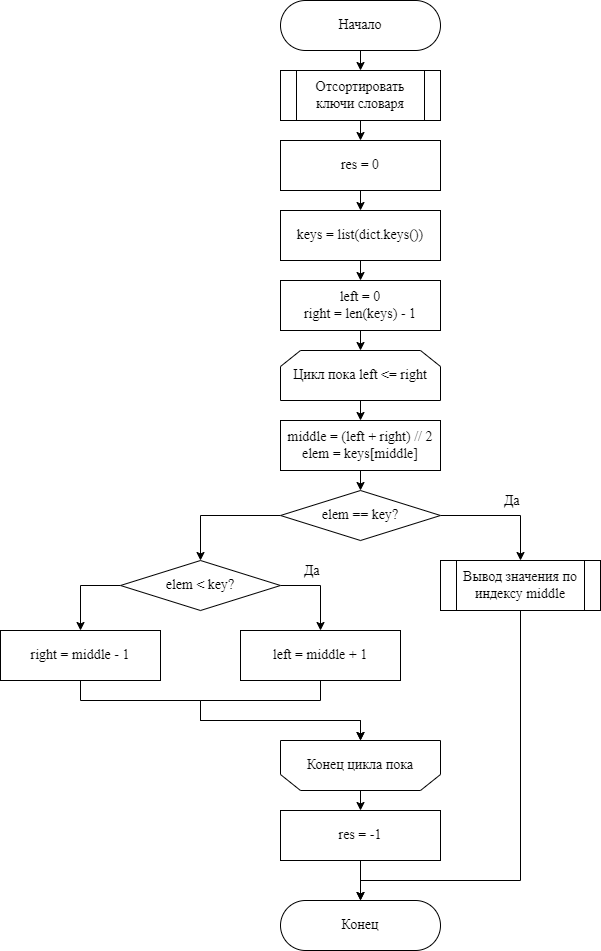
\includegraphics[width=380pt]{inc/bin_search.png}
	\caption{Алгоритм бинарного поиска}
	\label{fig:bin-search}	
\end{figure}

\clearpage

\begin{figure}[h!btp]
	\centering
	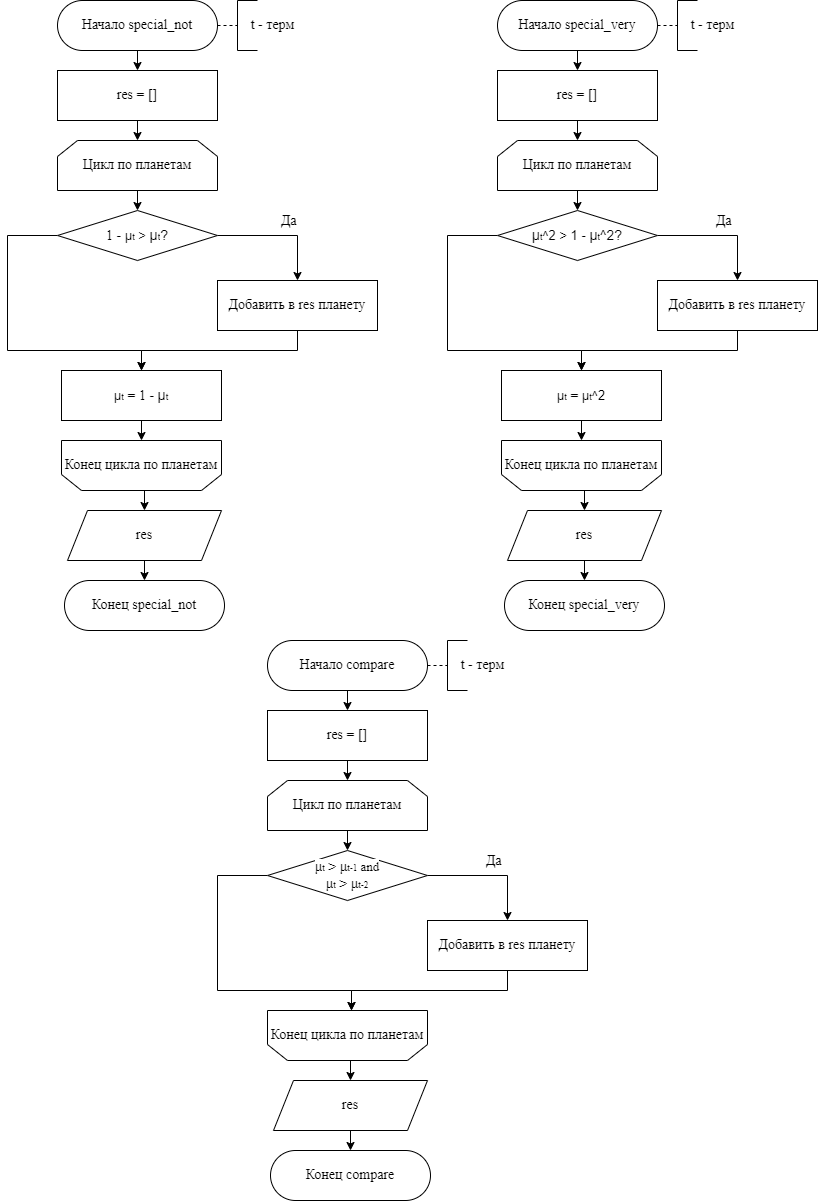
\includegraphics[width=460pt]{inc/not_very.png}
	\caption{Алгоритмы получения объектов по значениям функций принадлежности}
	\label{fig:not-very}	
\end{figure}

\clearpage

\begin{figure}[h!btp]
	\centering
	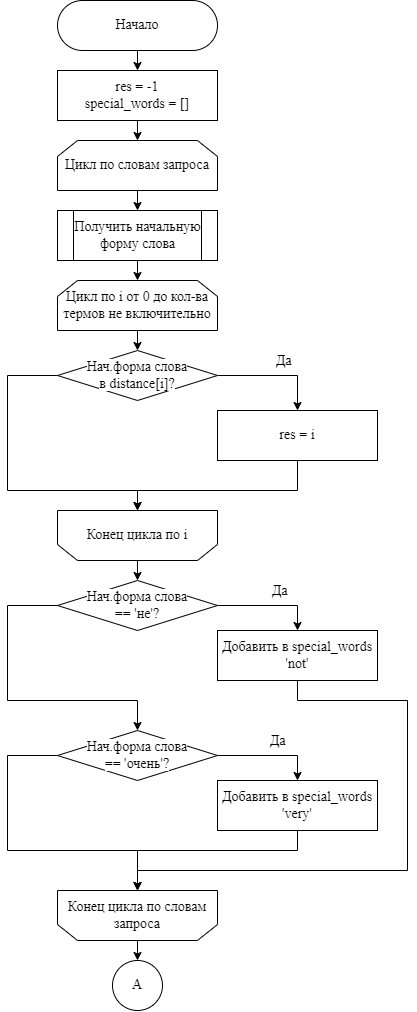
\includegraphics[width=280pt]{inc/get_planets_1.png}
	\caption{Алгоритм получения объектов по ограничению}
	\label{fig:get1}	
\end{figure}

\clearpage

\begin{figure}[h!btp]
	\centering
	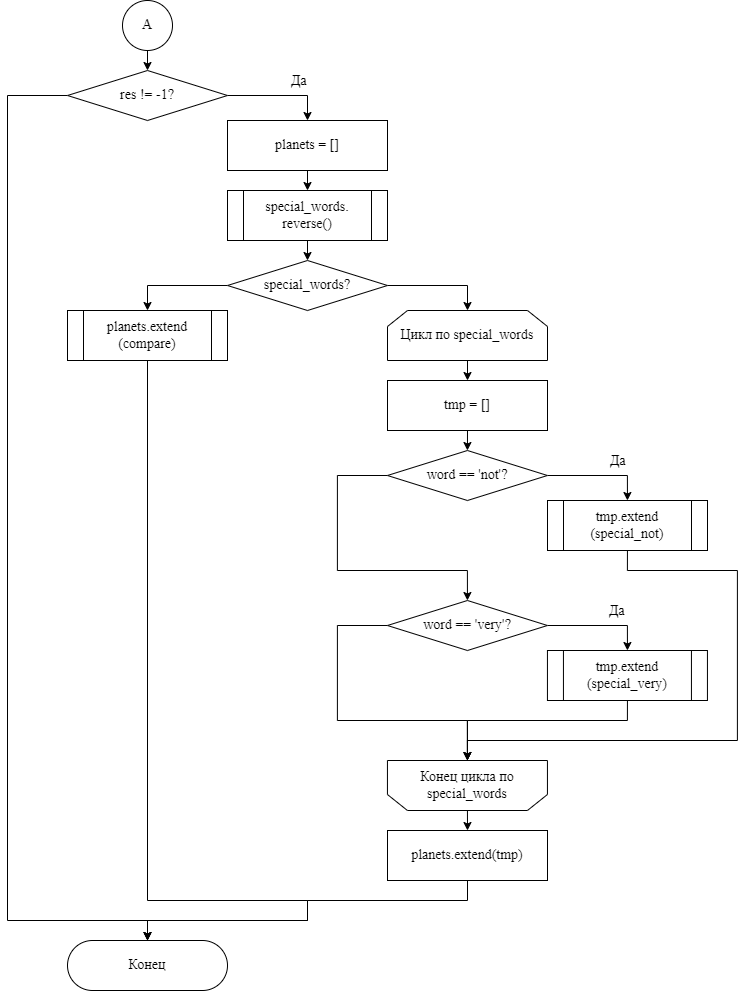
\includegraphics[width=460pt]{inc/get_planets_2.png}
	\caption{Алгоритм получения объектов по ограничению (продолжение)}
	\label{fig:get2}	
\end{figure}

\clearpage

\vspace{\baselineskip}
\subsection*{Вывод}
\vspace{\baselineskip}

Были разработаны алгоритмы бинарного поиска и получения объектов по заданному в вопросе на естественном языке ограничению.
